\documentclass[12pt]{article}

\usepackage{fixltx2e}
\usepackage{textcomp}
\usepackage{fullpage}
\usepackage{amsfonts}
\usepackage{verbatim}
\usepackage[english]{babel}
\usepackage{pifont}
\usepackage{color}
\usepackage{setspace}
\usepackage{lscape}
\usepackage{indentfirst}
\usepackage[normalem]{ulem}
\usepackage{booktabs}
% \usepackage{nag}
\usepackage{natbib}
% \usepackage{bibtex}
\usepackage{float}
\usepackage{latexsym}
\usepackage{hyperref}
\usepackage{url}
% \usepackage{html}
\usepackage{epsfig}
\usepackage{graphicx}
\usepackage{amssymb}
\usepackage{amsmath}
\usepackage{bm}
\usepackage{array}
%\usepackage{mhchem}
\usepackage{ifthen}
\usepackage{caption}
\usepackage{xcolor}
\usepackage{amsthm}
\usepackage{amstext}
\usepackage{nicefrac}
\usepackage{algorithm}
\usepackage{algorithmic}
\usepackage[scientific-notation=true]{siunitx}
\usepackage{subfigure}
\usepackage[flushleft]{threeparttable}
\usepackage{lineno}
\usepackage{adjustbox}
\usepackage{ragged2e}
\usepackage{authblk}

\setlength{\parskip}{1em}
\renewcommand{\baselinestretch}{2.0}
\renewcommand\Affilfont{\small}

\begin{document}

\title{StarBEAST2 enables accurate and precise inference of species trees, divergence times and clock rates}
\author[1,2]{Huw A. Ogilvie\thanks{huw.ogilvie@anu.edu.au}}
\author[2,3]{Alexei J. Drummond}
\affil[1]{Division of Evolution, Ecology and Genetics, Research School of Biology, Australian National University, Canberra, Australia}
\affil[2]{Centre for Computational Evolution, University of Auckland, Auckland, New Zealand}
\affil[3]{Department of Computer Science, University of Auckland, Auckland, New Zealand}

\maketitle

\clearpage

\justifying

\section{Abstract}

Keywords: Phylogenetic methods, substitution rate, relaxed clock, multispecies coalescent, concatenation.

\section{Introduction}


\section{New Approaches}

\subsection{Coordinated tree changing operators}

\subsection{Species tree relaxed clocks}

\section{Results}

\subsection{StarBEAST2 correctly implements the multispecies coalescent}

New methods must be shown to be mathematically correct implementations of a
given model. One way to accomplish this for MCMC methods is to estimate
parameters from a prior distribution using the MCMC kernel, and also draw
independent samples from the same prior distribution by simulation. The
resulting parameter distributions should be identical if the implementation is
correct. We used this method to test the correctness of the novel features in
StarBEAST2; analytical population size integration, the four new operators, and
the species tree relaxed clock. Simulated and StarBEAST2 estimated distributions
were identical for species and gene tree topologies (Figure~S1,S2), species and
gene tree node heights (Figure~S3,S4) and gene tree branch rates (Figure~S5).
This combination of results supports the mathematical correctness of StarBEAST2.

\subsection{\textit{Pseudacris} chorus frogs have intermediate coalescent branch lengths}

To characterize the performance of new operators, methods of population size
integration and relaxed cocks, we tested StarBEAST2 using real sequence data.
The data set used for this analysis is from the North American chorus frog genus
\textit{Pseudacris}, and was originally collected and analyzed by
\cite{Barrow201478}. A key metric of phylogenies that can be used to judge
whether it is necessary to employ multispecies coalescent models is the average
branch length in coalescent units of $\nicefrac{\tau}{2Ne}$. Given short branch
lengths, concatenation is unable to infer accurate species trees regardless of
the number of loci used, but for long branch lengths, concatenation is
approximately as accurate as *BEAST \citep{Ogilvie01052016}. Using StarBEAST2,
the average branch length within this genus was determined to be
$\nicefrac{1.69\tau}{2Ne}$. This is an intermediate average length, longer than
the shallow simulations analyzed by \cite{Ogilvie01052016}, which had short
branch lengths of $\nicefrac{0.54\tau}{2Ne}$.

\subsection{New operators and analytical integration improve computational performance}

To determine which configuration of new features would achieve the fastest
performance, we ran StarBEAST2 using different combinations of new operators,
analytical integration of population sizes and relaxed clocks. To measure
convergence both effective sample size (ESS) per hour and ESS per million states
were computed for each independent chain. ESS per hour can be used calculate the
total time required for a converged chain where ESS is equal to or above 200,
and reflects the efficiency of new state proposals and the computational time
required by each operator and likelihood calculation. In contrast, ESS per
million states reflects only to the efficency of new state proposals,
independent of calculation times. A variety of statistics were logged for each
analysis, but the height of the species tree had the slowest convergence rates
so we used this statistic to judge computational performance (Figure~S7-Sx).

Coordinated topology operators consistently reduced ESS per hour convergence,
regardless of the addition of height changing operators or the method of
population size integration (Figure~\ref{fig:realEssPerHour}). However these
operators had little effect on ESS per million states (Figure~\ref{fig:realEssPerMstates}).
The latter result suggests that coordinated topology operators are not more
effective than na\"ive operators at proposing new states, and the former result
shows how the increased complexity of these operators harms convergence because
of their increased computational time cost.

\begin{figure}[htb!]
\centering
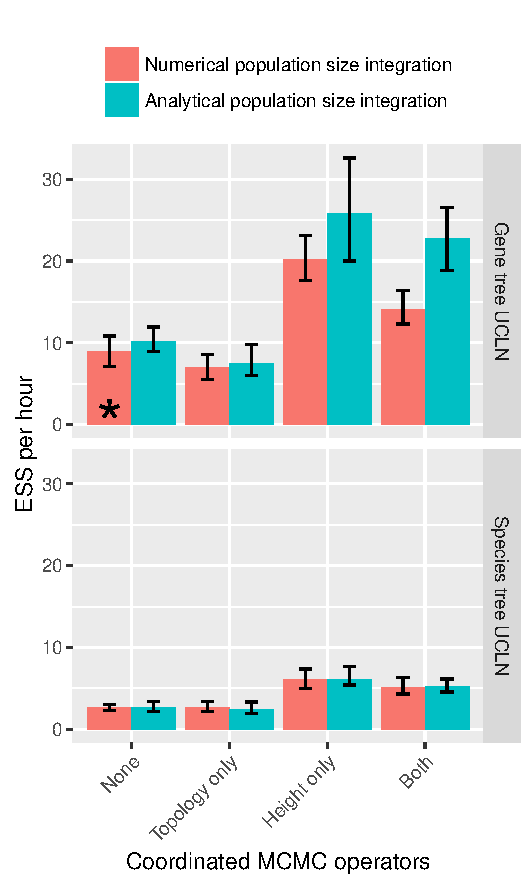
\includegraphics[height=14cm]{speciesTreeHeight_ess_per_hour.pdf}
\caption
{Effect of operators, population size integration and clock models on
convergence. The performance of every combination of settings was measured when
applied to 22 \textit{Pseudacris} loci. Topology operators refers to the
replacement of na\"ive NNI and SPR operators with coordinated operators. Heights
operators refers to the addition of operators which make coordinated changes to
internal node heights. Uncorrelated lognormal (UCLN) relaxed clocks were applied
to either each gene tree or to the species tree. Trimmed means of species tree
height effective sample size (ESS) per hour were calculated from 32 independent
chains. 25\% trim was used to reduce the influence of outliers. All error bars
are 95\% confidence intervals calculated by bootstrapping.}
\label{fig:realEssPerHour}
\end{figure}

\begin{figure}[htb!]
\centering
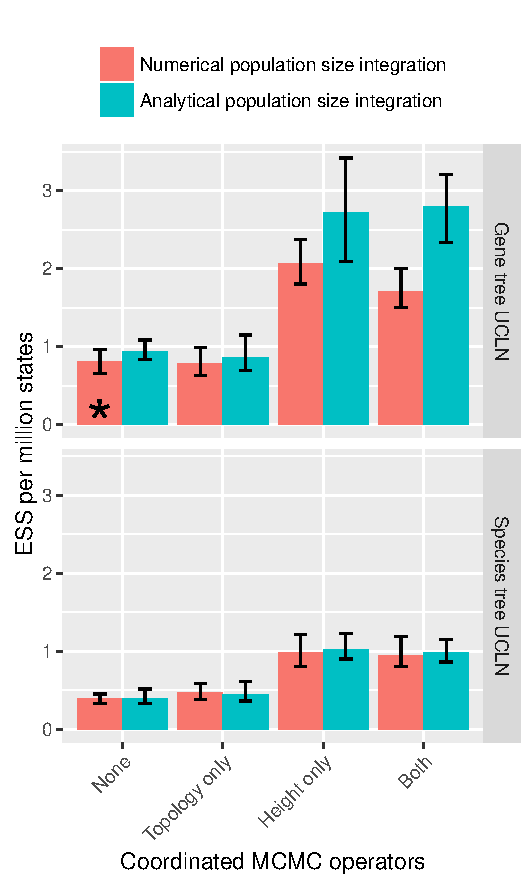
\includegraphics[height=14cm]{speciesTreeHeight_ess_per_mstates.pdf}
\caption
{Effect of operators, population size integration and clock models on effective
sample size (ESS) per million states. The performance of every combination of
settings was measured when applied to 22 \textit{Pseudacris} loci. Topology operators refers to the
replacement of na\"ive NNI and SPR operators with coordinated operators. Heights
operators refers to the addition of operators which make coordinated changes to
internal node heights. Uncorrelated lognormal (UCLN) relaxed clocks were applied
to either each gene tree or to the species tree. Trimmed means
of species tree height ESS per million states were calculated from 32
independent chains. 25\% trim was used to reduce the influence
of outliers. All error bars are 95\% confidence intervals calculated by
bootstrapping.}
\label{fig:realEssPerMstates}
\end{figure}

Coordinated height changing operators consistently improved convergence both in
terms of ESS per hour and ESS per million states
(Figure~\ref{fig:realEssPerHour},\ref{fig:realEssPerMstates}). Both species tree
relaxed clock and gene tree relaxed clock analyses benefitted from enabling
these new operators. Unlike height changing operators analytical integration of
population sizes only improved the computational performance of gene tree
relaxed clock analyses, not the performance of species tree relaxed clock
analyses.

Convergence of species tree relaxed clock analyses was dramatically slower than
convergence of gene tree relaxed clock analyses. The relative performance in ESS
per hour was worse than the relative performance in ESS per million states
(Figure~\ref{fig:realEssPerHour},\ref{fig:realEssPerMstates}), which shows that
compared to gene tree relaxed clock analyses the likelihood calculations have a
higher time cost, but also that new state proposals are less effective at
exploring the space of phylogenies and parameters.

\subsection{StarBEAST2 is approximately three times faster than *BEAST}

Our reanalysis of \textit{Pseudacris} sequence data shows that analytical
integration of population sizes and coordinated height changing operators both
improve convergence. To show that this increased performance is generally
applicable, and to demonstrate that StarBEAST2 can accurately reconstruct branch
rates under a species tree relaxed clock model, we needed to apply StarBEAST2 to
many different data sets for which the true species tree is known. Therefore we
simulated 64 species trees of 19 taxa each under a birth-death model with
lognormally distributed branch rates. Gene trees evolving within each species
tree were simulated according to the multispecies coalescent model with
lognormally distributed mean clock rates. Finally, sequences were simulated
according to an HKY+$\Gamma$ process for each gene. The parameters used for
these simulations were chosen to also produce intermediate branch lengths in
coalescent units; the average branch length was $\nicefrac{1.44\tau}{2Ne}$.

StarBEAST2 with *BEAST settings --- explicit MCMC integration of population
sizes, no coordinated operators, na\"ive NNI and SPR topology operators, and a
UCLN relaxed clock applied to each gene tree. StarBEAST2 with performant
settings --- analytical integration of population sizes, coordinated height
changing operators and na\"ive NNI and SPR topology operators --- and a UCLN
relaxed clock applied to each gene tree or alternatively to the species tree.

Again the parameter with the slowest convergence for any multispecies coalescent
settings was the height of the species tree. Based on that parameter, the
average performance increase using StarBEAST2 with performant settings over
*BEAST settings was 3.2 times, with a 95\% confidence interval between 2.6 and
3.8 (Figure~\ref{fig:simulatedEssPerHour}). The slowest converging parameter for
concatenated analyses was the posterior log-probability. Using the same number
of loci, the convergence of the posterior statistic using concatenation was
114.5 times faster than the convergence of the species tree height statistic
using StarBEAST2 with *BEAST settings. When concatenation was used with ten
times the number of loci, the performance difference was minimal --- 1.2 times,
with a confidence interval between 1.0 and 1.5 times
(Figure~\ref{fig:simulatedEssPerHour}).

Unlike the real data, using a species tree UCLN relaxed clock with performant
settings was faster than *BEAST settings. However, this was still significantly
slower than using gene tree relaxed clocks, as the average performance increase
was smaller at 1.5 times with a confidence interval between 1.2 and 1.9
(Figure~\ref{fig:simulatedEssPerHour}).

\begin{figure}[htb!]
\centering
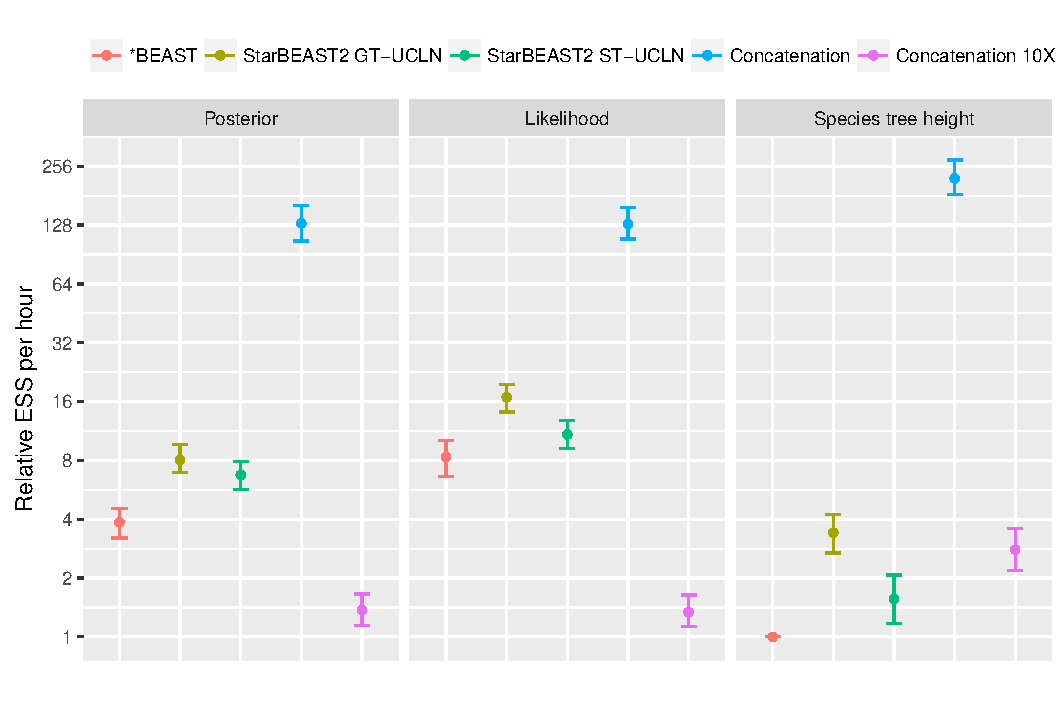
\includegraphics[width=16cm]{multiple_ess_per_hour.pdf}
\caption
{Convergence of different methods applied to simulated data. Methods are
concatenation with 22 loci, concatenation with 220 loci (10X), StarBEAST2 with
*BEAST settings and 22 loci, and StarBEAST2 with performant settings, 22 loci,
and uncorrelated lognormal relaxed clocks applied to the gene tree (GT-UCLN) or
to the species tree (ST-UCLN). Relative ESS per hour is the trimmed mean of
effective sample size per hour for each replicate divided by the slowest rate
(the species tree height estimated using *BEAST
settings). 25\% trim was used to reduce the influence of
outliers. All error bars are 95\% confidence intervals calculated by
bootstrapping. N = 64.}
\label{fig:simulatedEssPerHour}
\end{figure}

\subsection{The relative accuracy of StarBEAST2 varies depending on metric}

The accuracy of StarBEAST2 relative to concatenation varied depending on the
metric used and whether equal numbers of loci were used. Relative species tree
error measures the accuracy of estimated branch lengths; StarBEAST2 using 22
loci outperformed concatenation using 22 loci, and matched the performance of
concatenation using 220 loci (Figure~\ref{fig:speciesTreeError}A). Pendant
edge bias measures systematic bias in the estimated ages of extant species;
StarBEAST2 was much less biased than concatenation regardless of the number of loci
(Figure~\ref{fig:speciesTreeError}B). Rooted Robinson-Foulds distances measure
the topological accuracy of estimated trees; concatenation using 22 loci was
almost as accurate as StarBEAST2, and much more accurate when using 220 loci
(Figure~\ref{fig:speciesTreeError}C). For no metric did the choice of gene tree
or species tree relaxed clocks change the accuracy of StarBEAST2
(Figure~\ref{fig:speciesTreeError}A,B,C).

\begin{figure}[htb!]
\centering
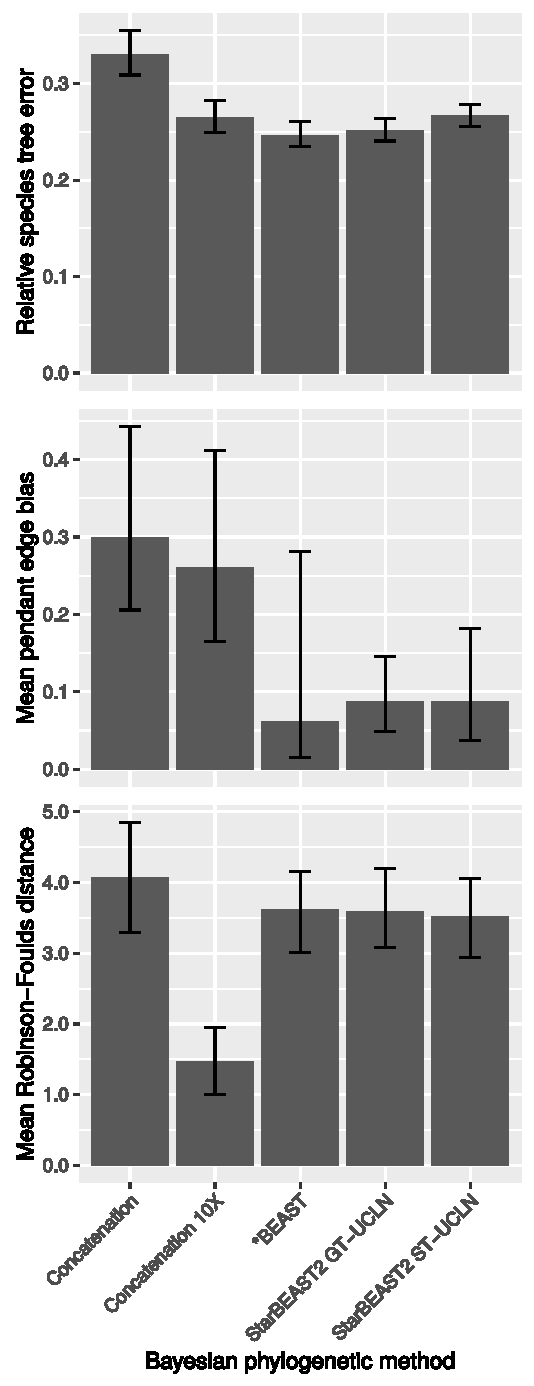
\includegraphics[width=6.5cm]{tree_error.pdf}
\caption
{Accuracy of different methods applied to simulated data. Methods are concatenation with 22 loci, concatenation with 220 loci
(10X), StarBEAST2 with *BEAST settings and 22 loci, and StarBEAST2 with
performant settings, 22 loci, and uncorrelated lognormal relaxed clocks applied
to the gene tree (GT-UCLN) or to the species tree (ST-UCLN). (A) Trimmed mean of
relative species tree error, a measure of branch length error. (B) Trimmed
mean of mean pendant edge bias, which measures biased estimates of the ages of
extant species. (C) Trimmed mean of mean rooted Robinson-Foulds distances, a
measure of topological error. 25\% trim was used to reduce the
influence of outliers. All error bars are 95\% confidence intervals calculated
by bootstrapping. N = 64.}
\label{fig:speciesTreeError}
\end{figure}

\subsection{Concatenation cannot reconstruct branch rates given intermediate branch lengths}

While the convergence of species tree relaxed clocks analyses was slower than gene tree
relaxed clock analyses using StarBEAST2, species tree relaxed clocks enable inference of per-branch
substitution rates under the multispecies coalescent model. To gauge the
accuracy of estimated branch rates, we used simple linear regression (SLR)
models with the true rate of each simulated branch as the response variable, and
the posterior expectation of the rate of that branch (conditional on the
corresponding clade being monophyletic in the posterior sample) as the
explanatory variable (Figure~\ref{fig:branchRatesLM}). If all estimates equal
the truth, then the $R^2$ correlation coefficient of the SLR will equal 1, the
slope of the SLR will also equal 1, and the intercept will equal zero.

Using either 22 or 220 loci, concatenation was unable to correctly estimate
branch lengths --- not only did $R^2 = 0.03$ and $0.04$ respectively, but the
slope and intercept were $0.32x + 0.68$ and $0.79x + 0.21$ respectively. By
applying a UCLN relaxed clock to the species tree, StarBEAST2 can be used to
infer many branch rates --- the $R^2$ correlation was much stronger at $0.15$,
and the slope and intercept were $0.93$ and $0.07$ respectively, much closer to
the ideal values (Table~\ref{tab:branchRatesLM}).

\begin{figure}[htb!]
\centering
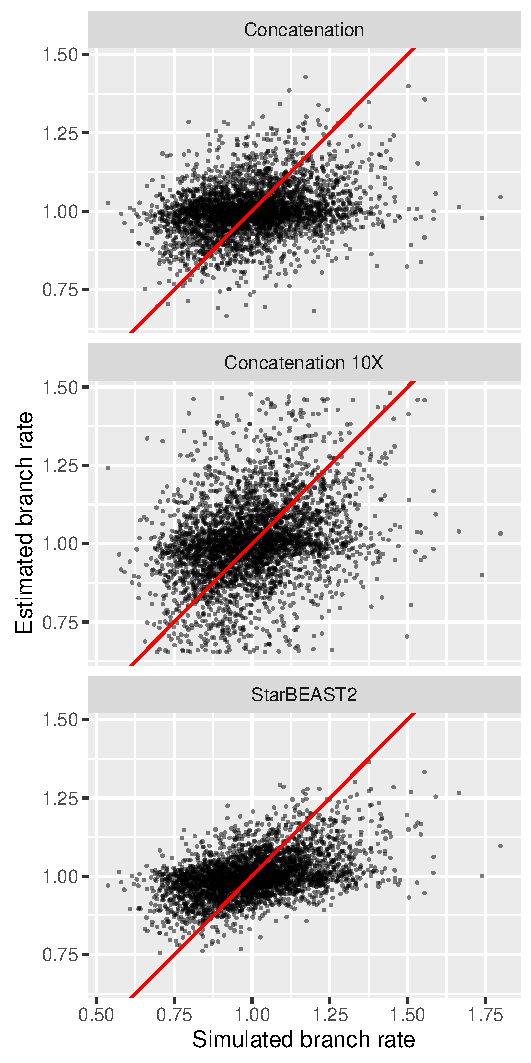
\includegraphics[width=16cm]{branch_rates.pdf}
\caption
{Recovery of species tree branch rates using concatenation and StarBEAST2.
Methods are concatenation with 22 loci, concatenation with 220 loci (10X), and
StarBEAST2 with performant settings, 22 loci, and an uncorrelated lognormal
relaxed clocks applied to the species tree (ST-UCLN). Estimated rates are the
posterior expectation of the branch rate. $R^2$ values and lines of best fit were calculating using a separate
simple linear regression for each method. Root branch rates, which were fixed at
1.0, were excluded. N = 64.}
\label{fig:branchRatesLM}
\end{figure}

\begin{table}[htb!]
\centering
\caption{Simple linear regression of simulated and estimated species tree branch rates.}
\label{tab:branchRatesLM}
\begin{threeparttable}
\begin{adjustbox}{center}
\small
$\begin{array}{|c|c|l|l|l|}
\multicolumn{1}{c}{\text{Method}} & \multicolumn{1}{c}{\text{Number of loci}} & \multicolumn{1}{c}{\text{Intercept}} & \multicolumn{1}{c}{\text{Slope}} & \multicolumn{1}{c}{R^2}\tabularnewline
\hline
\text{Concatenation} & 22 & 0.68^{***} & 0.32^{***} & 0.03\tabularnewline
\hline
\text{Concatenation} & 220 & 0.79^{***} & 0.21^{***} & 0.04\tabularnewline
\hline
\text{StarBEAST2} & 22 & 0.07 & 0.93^{***} & 0.15\tabularnewline
\hline
\end{array}$
\end{adjustbox}
\begin{tablenotes}
\small
\item {*}: $p < 0.05$, {**}: $p < 0.01$, {***}: $p < 0.001$.
\end{tablenotes}
\end{threeparttable}
\end{table}

\clearpage

\section{Discussion}


\section{Materials and Methods}


\section{Supplementary Material}

%Supplementary tables XX-XX and figures XX-XX are available at \textit{Molecular Biology and Evolution} online (http://www.mbe.oxfordjournals.org/).
Supplementary tables and figures will be available online.

\section{Acknowledgments}

This work was supported by a Rutherford Discovery Fellowship awarded to AJD by
the Royal Society of New Zealand. HAO was supported by an Australian Laureate
Fellowship awarded to Craig Moritz by the Australian Research Council
(FL110100104). This research was undertaken with the assistance of resources
from the National Computational Infrastructure (NCI), which is supported by the
Australian Government. We wish to thank Jason Bragg for help testing StarBEAST2,
and Tim Vaughan for suggesting the addition of the root height changing
operator. We also wish to thank Joseph Heled for insight into the multispecies
coalescent model, and Graham Jones for input regarding operator performance.

\bibliographystyle{natbib}
\bibliography{starbeast2}

\end{document}
